\chapter{Introducción}\label{chapter:introduction}
\addcontentsline{toc}{chapter}{Introducción}

La medicina moderna ha fortalecido el control de enfermedades mediante el desarrollo de vacunas. Sin embargo, su aplicación masiva en la población exige garantizar su seguridad de manera rigurosa y continua.
Esta exigencia se materializa en un proceso escalonado de investigación clínica, que transcurre por diversas etapas antes de la aprobación del fármaco, tal como se ilustra en la Figura \ref{fig:desarrollo_clinico}.

En las etapas I, II y III, el producto se somete a estudios controlados en grupos seleccionados de voluntarios para reunir datos preliminares sobre su seguridad y definir las recomendaciones de posología y eficacia a corto plazo. 
Durante estas fases, el producto biológico permanece en un entorno científico resguardado, donde la población de estudio es reducida (rara vez superando los 5,000 sujetos) y generalmente homogénea, lo que limita la detección de reacciones poco frecuentes \cite{who_pharmacovigilance_2004}.

\begin{figure}[htbp]
    \centering
    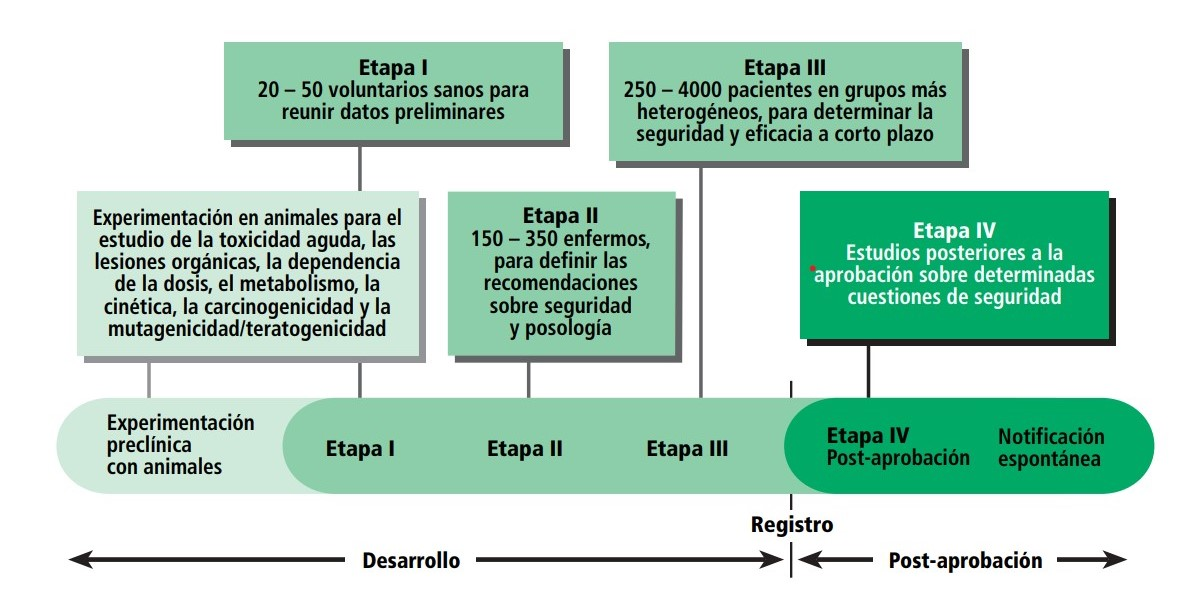
\includegraphics[width=0.8\textwidth]{Graphics/Cap1/fig1_desarrollo_clinico.jpg}
    \caption{Etapas del desarrollo clínico de vacunas. Adaptado de \cite{who_pharmacovigilance_2004}.}
    \label{fig:desarrollo_clinico}
\end{figure}

Una vez que la \gls{vacuna} recibe el registro sanitario y comienza su uso masivo en la población general, se inicia la etapa IV o post-aprobación. 
En estas condiciones reales de uso, el escenario cambia drásticamente: el producto se administra a grupos diversos que incluyen niños, ancianos, embarazadas y personas con múltiples patologías, quienes a menudo fueron excluidos de los ensayos iniciales \cite{who_pharmacovigilance_2004}.

Precisamente en esta fase es donde comienzan a manifestarse los Eventos Supuestamente Atribuibles a la Inmunización (ESAVI), definidos como cualquier cuadro clínico desfavorable (signo, síntoma o enfermedad) que ocurre tras la vacunación y no necesariamente tiene una relación causal con la vacuna \cite{paho_curso_esavi}.

Para gestionar estos riesgos inevitables, surge la \gls{farmacovigilancia} como la ciencia y las actividades relativas a la detección, evaluación, comprensión y prevención de los efectos adversos de los medicamentos.
Esta disciplina permite evaluar continuamente la relación beneficio-riesgo y detectar señales de alerta que no fueron identificadas durante las fases iniciales de investigación \cite{who_pharmacovigilance_2004}.

\section{Contexto histórico y social de la farmacovigilancia}\label{section:contextoHistoricoSocial}



% La evolución de la farmacovigilancia ha estado marcada por eventos históricos en los que las herramientas clínicas disponibles resultaron insuficientes para detectar oportunamente riesgos asociados al uso de medicamentos. Entre los principales hitos se encuentran el caso de Hannah Greener en 1848, cuya muerte bajo anestesia con cloroformo originó los primeros intentos de notificación voluntaria de reacciones adversas \cite{historia_farmacovigilancia_2023}; la tragedia del Elíxir de Sulfanilamida en 1937, que provocó más de 100 muertes infantiles y llevó al refuerzo de la regulación de la \gls{fda} \cite{historia_farmacovigilancia_2023}; y el desastre de la talidomida en 1961, una epidemia de focomelia que causó más de 10,000 casos de malformaciones congénitas y consolidó la necesidad de sistemas formales de vigilancia \cite{tarrago_farmacovigilancia_cuba_2019,palacios2021talidomida}.

% Como respuesta a esta última catástrofe, la Organización Mundial de la Salud (\gls{oms}) impulsó en 1963 la creación de mecanismos internacionales para la comunicación rápida de reacciones adversas \cite{historia_farmacovigilancia_2023}, lo que dio origen en 1968 al Programa Internacional de Monitoreo de Medicamentos (\gls{pimm}). 
% Este programa permitió la recolección y análisis conjunto de notificaciones a nivel global para la detección de señales de riesgo \cite{who_pharmacovigilance_2004}. 
% Posteriormente, en 1978 se estableció el Centro de Monitoreo de Uppsala (\gls{umc}), encargado de proporcionar liderazgo científico y apoyo operativo al programa de la \gls{oms} \cite{barrero2022notificacion}.

% Antes de la digitalización, la vigilancia se basaba en sistemas de notificación en papel, destacando la “Tarjeta Amarilla” implementada en el Reino Unido en 1964, que permitía a los profesionales sanitarios reportar sospechas de reacciones adversas mediante \gls{formularios} estandarizados \cite{historia_farmacovigilancia_2023,normas_farmacovigilancia_cuba_2012}. Este modelo fue adoptado internacionalmente como base de los sistemas de notificación.

% La gestión de datos evolucionó desde el reporte manual en tarjetas amarillas hacia \gls{repositorios} mundiales como \gls{VigiBase}, que hoy centraliza más de 20 millones de registros. 
% Semejante volumen de información hizo indispensable la automatización mediante sistemas como \gls{faers} y ecosistemas inteligentes como \gls{aems}, capaces de procesar flujos masivos de datos con una agilidad inalcanzable para los métodos tradicionales.

La evolución de la farmacovigilancia ha estado marcada por tragedias sanitarias —como el desastre de la talidomida en 1961— que evidenciaron la necesidad de sistemas formales de vigilancia\cite{tarrago_farmacovigilancia_cuba_2019,palacios2021talidomida}. 
Como respuesta, la Organización Mundial de la Salud (\gls{oms}) impulsó mecanismos internacionales que dieron origen al Centro de Monitoreo de Uppsala \cite{barrero2022notificacion}. 
Desde los primeros intentos de notificación voluntaria y el modelo de la Tarjeta Amarilla (ver glosario \gls{tarjeta_amarilla}) en papel, se ha transitado hacia repositorios globales como VigiBase (ver glosario \gls{VigiBase}), que centraliza más de 20 millones de registros y exige la automatización para procesar flujos masivos de datos.


\subsubsection*{La farmacovigilancia en Cuba}

% Cuba posee una sólida trayectoria institucional en materia de seguridad de medicamentos, integrándose formalmente al Programa Internacional de Monitoreo de Medicamentos de la \gls{oms} en 1994 \cite{paho_vigilancia_medicamentos_cuba}.

% Posteriormente, en 1999, se consolidó el actual Sistema Cubano de Farmacovigilancia (\gls{scfv}), bajo la rectoría de la Unidad Coordinadora Nacional de Farmacovigilancia (\gls{ucnfv}), con el objetivo de unificar los métodos de validación e identificación de riesgos en todo el territorio nacional \cite{tarrago_farmacovigilancia_cuba_2019}.

% En cuanto al comportamiento de los indicadores, el sistema cubano presenta niveles de desempeño superiores a los estándares internacionales. 
% Mientras que la tasa de reporte considerada eficiente a nivel mundial oscila entre 250 y 300 notificaciones por millón de habitantes al año, Cuba ha mantenido históricamente cifras muy por encima de este umbral \cite{cecmed_farmacovigilancia_cuba_2020}. 
% Por ejemplo, en el año 2020, se recibieron un total de 13,025 reportes, lo que representa una tasa de 1,163 por millón de habitantes, como se muestra en la Figura \ref{fig:ram_eventos_adversos_cuba_2020} .

% \begin{figure}[htbp]
%     \centering
%     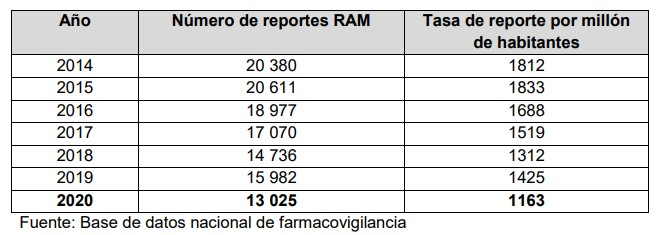
\includegraphics[scale=1.2]{Graphics/Cap1/ram_en_cuba_2020.jpg}
%     \caption{Reporte de \gls{reacción adversa a medicamentos (RAM)}. Fuente: \gls{cecmed} en su informe anual del año 2020 \cite{cecmed_farmacovigilancia_cuba_2020}.}
%     \label{fig:ram_eventos_adversos_cuba_2020}
% \end{figure}


Cuba posee una sólida trayectoria en seguridad de medicamentos, integrándose al Programa Internacional de Monitoreo de Medicamentos de la \gls{oms} en 1994 y consolidando su Sistema Cubano de Farmacovigilancia (\gls{scfv}) en 1999 \cite{paho_vigilancia_medicamentos_cuba, tarrago_farmacovigilancia_cuba_2019}.

El sistema cubano presenta niveles de desempeño superiores a los estándares internacionales. Mientras la tasa eficiente global oscila entre 250 y 300 notificaciones por millón de habitantes al año, Cuba alcanzó en 2020 un total de 13,025 reportes, lo que representa una tasa de 1,163 por millón de habitantes \cite{cecmed_farmacovigilancia_cuba_2020} (véase Anexo \ref{app:reportes_cuba_2020}).


% \paragraph{IMPORTANTE}

% Sin embargo, al analizar la distribución de estos reportes por grupo farmacológico, se observa que la mayoría se concentra en medicamentos de uso frecuente como antibacterianos, antihipertensivos y analgésicos. 
% En contraste, los eventos asociados a vacunas representan una proporción considerablemente menor dentro del total de notificaciones, con alrededor de 700 reportes, como se evidencia en la Figura \ref{fig:RAM_por_grupo_farmacologico_cuba_2020}. 

% \begin{figure}[htbp]
%     \centering
%     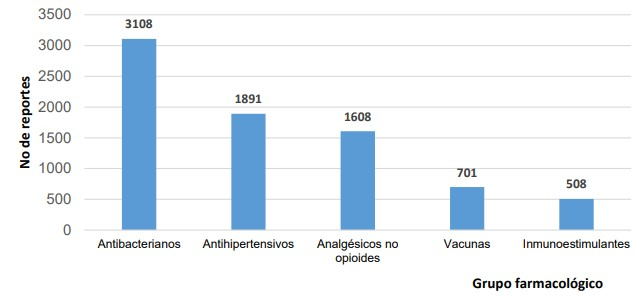
\includegraphics[scale=1.2]{Graphics/Cap1/grupo_farmacologico.jpg}
%     \caption{Reporte de \gls{reacción adversa a medicamentos (RAM)} según grupo farmacológico. Farmacovigilancia pasiva 2020.}
%     \label{fig:RAM_por_grupo_farmacologico_cuba_2020}
% \end{figure}

% Durante la primera década del siglo XXI y los primeros años de la segunda, Cuba alcanzó un desempeño destacado en farmacovigilancia, situándose entre los 20 países con mayores tasas de notificación de \gls{reacción adversa a medicamentos (RAM)} por millón de habitantes a nivel mundial \cite{normas_farmacovigilancia_cuba_2012}. 
% En el ámbito específico de la inmunización, mediante su sistema de vigilancia de \gls{esavi}, Cuba ocupó en 2018 el tercer lugar en la región de las Américas por volumen de notificaciones, con 6,682 reportes \cite{ops_manual_esavi_2021}. 
% Esto la sitúa solo por detrás de países como Estados Unidos y Brasil, como se muestra en la Figura \ref{fig:esavi_por_paises}.

% \begin{figure}[H]
%     \centering
%     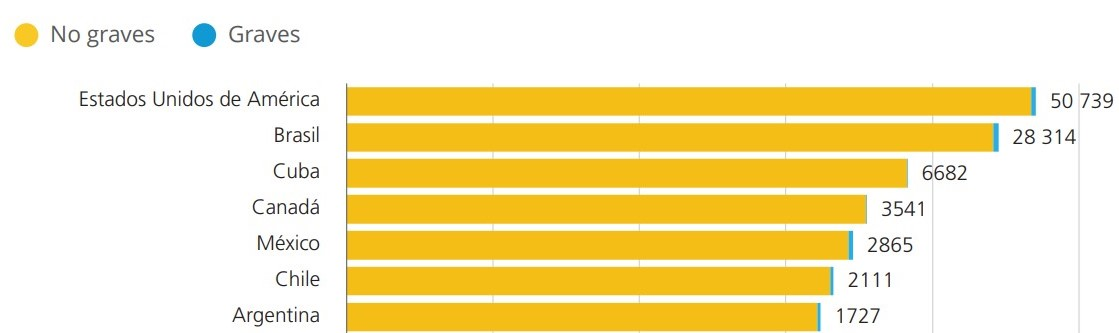
\includegraphics[scale=0.6]{Graphics/Cap1/copia_paises_ram.jpg}
%     \caption{Número de \gls{esavi} notificados por los países de la región de las Américas}
%     \label{fig:esavi_por_paises}
% \end{figure}


Sin embargo, al analizar la distribución por grupo farmacológico en el propio año, la mayoría de los reportes se concentra en medicamentos de uso frecuente (antibacterianos, antihipertensivos, analgésicos), mientras que los eventos asociados a vacunas representan una proporción menor, con alrededor de 700 reportes (véase Anexo \ref{app:grupo_farmacologico}).

Cuba durante este siglo ha alcanzado un desempeño destacado en farmacovigilancia, situándose entre los 20 países con mayores tasas de notificación a nivel mundial \cite{normas_farmacovigilancia_cuba_2012}. 
En el ámbito específico de las vacunas, mediante su sistema de vigilancia de \gls{esavi}, Cuba ocupó en 2018 el tercer lugar en la región de las Américas por volumen de notificaciones, con 6,682 reportes, solo detrás de Estados Unidos y Brasil \cite{ops_manual_esavi_2021} (véase Anexo \ref{app:esavi_por_paises}).


\subsubsection*{Estructura del sistema de vigilancia de medicamentos}

% El sistema de vigilancia de medicamentos en Cuba se estructura bajo la rectoría del \gls{cecmed}, autoridad reguladora nacional encargada de la evaluación, control y toma de decisiones sobre la seguridad de los medicamentos a partir de la información generada en el sistema.

% Para el cumplimiento de estas funciones, se articula una red de vigilancia integrada por diversos componentes que interactúan de manera coordinada (ver Figura \ref{fig:estructura_vigilancia_medicamentos_cuba}) \cite{paho_vigilancia_medicamentos_cuba}:

% \begin{figure}[htbp]
%     \centering
%     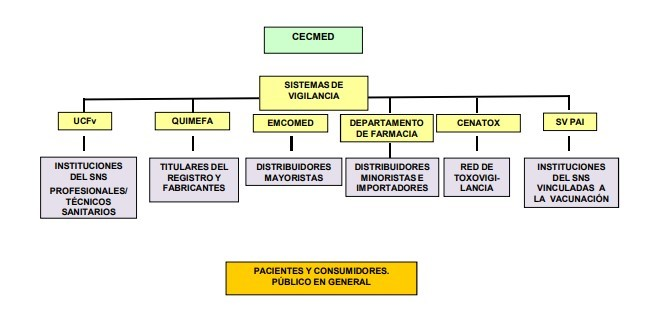
\includegraphics[scale=1.1]{Graphics/Cap1/estructura_vigilancia_medicamentos_cuba2.jpg}
%     \caption{Estructura del Sistema de Vigilancia de Medicamentos en Cuba.}
%     \label{fig:estructura_vigilancia_medicamentos_cuba}
% \end{figure}

% \begin{itemize} 
%     \item \textbf{\gls{ucnfv} (\gls{minsap}):} Cohesiona la Red de Farmacoepidemiología en los 169 municipios del país y actúa como el canal central para la \gls{notificación espontánea} de profesionales y pacientes, siendo las vacunas la excepción gestionada de forma especializada por el \gls{pai} \cite{paho_vigilancia_medicamentos_cuba,normas_farmacovigilancia_cuba_2012}. 
%     \item \textbf{Fabricantes y Titulares de Registro (QUIMEFA):} Involucra a las 24 empresas farmacéuticas nacionales, donde cada una cuenta con personal designado para la vigilancia y reporta directamente sobre la seguridad y calidad de sus productos \cite{paho_vigilancia_medicamentos_cuba}. 
%     \item \textbf{Distribución Mayorista (EMCOMED):} Coordina la vigilancia en las 24 droguerías del país, detectando problemas de calidad durante el almacenamiento y transportación \cite{paho_vigilancia_medicamentos_cuba}. 
%     \item \textbf{Distribución Minorista (Departamento de Farmacia):} Supervisa la vigilancia en las más de 2,000 farmacias comunitarias y hospitalarias del Sistema Nacional de Salud \cite{paho_vigilancia_medicamentos_cuba}.  
%     \item \textbf{\gls{cenatox}:} Lidera la red de toxicovigilancia, supervisando las intoxicaciones y reacciones adversas de naturaleza \gls{toxica} \cite{paho_vigilancia_medicamentos_cuba}. 
%     \item \textbf{SV \gls{pai}:} Realiza la vigilancia especializada de vacunas mediante el monitoreo de los \gls{esavi}, bajo la supervisión del Viceministerio de Higiene y Epidemiología \cite{paho_vigilancia_medicamentos_cuba}. 
% \end{itemize}

% Toda la información captada por estos efectores fluye hacia el Observatorio de Vigilancia Postcomercialización del \gls{cecmed}, donde se evalúa la relación beneficio-riesgo para emitir alertas farmacológicas, retirar lotes o modificar registros sanitarios en tiempo real \cite{paho_vigilancia_medicamentos_cuba}. 


El sistema de vigilancia de medicamentos en Cuba se estructura bajo la rectoría del \gls{cecmed}, con una red coordinada que integra a la \gls{ucnfv}, los fabricantes (QUIMEFA), las redes de distribución mayorista y minorista, el \gls{cenatox} y la vigilancia especializada de vacunas a cargo del \gls{pai} \cite{paho_vigilancia_medicamentos_cuba}. 
Toda la información fluye hacia el Observatorio de Vigilancia Postcomercialización del \gls{cecmed}, donde se evalúa la relación beneficio-riesgo para emitir alertas o retirar lotes (véase Anexo \ref{app:estructura_vigilancia}).


\subsubsection*{Instituto Finlay de Vacunas, fabricante líder del país}

El Instituto Finlay de Vacunas (\gls{ifv}) es una organización científica y empresa de alta tecnología cubana, integrada al Grupo \gls{biocubafarma}, que opera bajo un modelo de ciclo cerrado que abarca desde la investigación básica hasta la comercialización y el seguimiento postcomercialización \cite{finlay_instituto_2026}.

Como pilar estratégico de la soberanía tecnológica del país, el instituto garantiza la producción de 8 de las 11 vacunas administradas por el Programa Nacional de Inmunización, proveyendo el 78\% de las dosis totales del sistema de salud \cite{carbonell_cmi_finlay_2016}.

Su trayectoria de innovación incluye hitos científicos mundiales como la VA-MENGOC-BC® —primera vacuna eficaz contra el serogrupo B de la meningitis— y la Quimi-Hib, la primera vacuna conjugada con un antígeno totalmente sintético. 
Durante la crisis sanitaria global, el \gls{ifv} reafirmó su liderazgo al desarrollar la línea de vacunas SOBERANA contra la COVID-19, logrando una escala de operación sin precedentes con más de 38,7 millones de dosis administradas al cierre de julio de 2022 \cite{finlay_instituto_2026}. 
Internacionalmente, su prestigio se sustenta en exportaciones y colaboraciones estratégicas que impactan en más de 17 países de América Latina, Asia y África \cite{carbonell_cmi_finlay_2016}.



\section{Antecedentes, Motivación y Justificación}\label{section:antecedentesMotivacionJustificacion}


% Para la recogida y recolección de las sospechas de una respuesta nociva, el sistema emplea \gls{formularios} oficiales estandarizados que permiten captar la información mínima necesaria para el análisis clínico-epidemiológico y la detección precoz de riesgos.
% La Figura \ref{fig:flujo_farmacovigilancia_cuba} ilustra el flujo de la farmacovigilancia en Cuba que a continuación será descrito:


% \begin{itemize}
%     \item \textbf{Nivel de Base y Atención Primaria (Nivel Municipal):} El proceso se origina cuando un profesional sanitario (médico, enfermero, farmacéutico) o un paciente sospecha de una respuesta nociva o evento adverso tras la administración de un producto. 
%         \begin{itemize}
%             \item Para el registro de la sospecha de \gls{reacción adversa a medicamentos (RAM)}, los profesionales emplean el modelo oficial \textbf{33-36-02} (Anexo \ref{app:modelo_33-36-02}) y los pacientes el \textbf{33-36-03} (Anexo \ref{app:modelo_33-36-03}) \cite{normas_farmacovigilancia_cuba_2012}. 
%             \item En el caso específico de las vacunas, los profesionales deben utilizar obligatoriamente el modelo \textbf{84-30-2} (Anexo \ref{app:modelo_84-30-2}) para recopilar los datos técnicos del evento  \cite{normas_farmacovigilancia_cuba_2012, paho_vigilancia_medicamentos_cuba}.
%             \item En la comunidad, el reporte se entrega al jefe del grupo básico o al director técnico de la farmacia comunitaria, quienes lo remiten al farmacoepidemiológico municipal \cite{tarrago_farmacovigilancia_cuba_2019}.
%         \end{itemize}
%     \item \textbf{Nivel Provincial:} Las 16 unidades coordinadoras provinciales reciben las notificaciones de sus municipios \cite{normas_farmacovigilancia_cuba_2012}.
%         \begin{itemize}
%             \item Los especialistas provinciales evalúan la calidad del dato, codifican la información e introducen los reportes en su base de datos local \cite{normas_farmacovigilancia_cuba_2012}.
%             \item En casos de \gls{ram} \textbf{mortales o graves}, la notificación debe realizarse de forma inmediata (en menos de 24 horas) por vía telefónica o electrónica hacia el nivel nacional, procediendo a la custodias de muestras del fármaco para su investigación \cite{normas_farmacovigilancia_cuba_2012}.
%             \item El flujo regular de datos hacia la nación se realiza de manera quincenal (los días 15 y 30 de cada mes) \cite{normas_farmacovigilancia_cuba_2012}.
%         \end{itemize}
%     \item \textbf{Nivel Nacional y Gestión en FarmaVigiC:} La \gls{ucnfv}, ubicada en el Departamento de Farmacoepidemiología del \gls{minsap}, actúa como el órgano técnico-científico central \cite{tarrago_farmacovigilancia_cuba_2019}.
%         \begin{itemize}
%             \item Administra la base de datos nacional \gls{FarmaVigiC}, una herramienta informática que integra \textbf{75 variables} o campos críticos para el procesamiento de las notificaciones y el análisis clínico-epidemiológico (véase Anexo \ref{app:base_datos_farmavigic}) \cite{normas_farmacovigilancia_cuba_2012}.
%             \item Este nivel depura, valida y asigna puntajes de calidad a la información enviada por las provincias, consolidando el panorama nacional de seguridad farmacéutica \cite{normas_farmacovigilancia_cuba_2012}.
%             \item La \gls{ucnfv} coordina directamente con el \gls{cecmed} (Autoridad Reguladora Nacional) para la toma de medidas preventivas o alertas farmacológicas \cite{normas_farmacovigilancia_cuba_2012}.
%         \end{itemize}
%     \item \textbf{Vinculación Internacional (VigiBase):} Como miembro del Programa Internacional de Monitoreo de Medicamentos (\gls{pimm}):
%         \begin{itemize}
%             \item Los datos validados en la base nacional son extrapolados al formato internacional requerido, utilizando el diccionario \textbf{\gls{WHO-ART}} para la terminología de reacciones y el \textbf{\gls{ICD-10}} para la codificación de enfermedades \cite{normas_farmacovigilancia_cuba_2012}.
%             \item La \gls{ucnfv} remite trimestralmente todas las reacciones adversas importantes al \gls{umc} en Suecia, la cual alimenta a la base de datos \gls{VigiBase} \cite{normas_farmacovigilancia_cuba_2012}.
%         \end{itemize}
% \end{itemize}

% \begin{figure}[htbp]
%     \centering
%     \includegraphics[scale=0.20]{Graphics/Cap1/flujo_final_farma_cuba.png}
%     \caption{Flujo de la farmacovigilancia en Cuba para el reporte de \gls{esavi} }
%     \label{fig:flujo_farmacovigilancia_cuba}
% \end{figure}

% De forma transversal a estos niveles, los fabricantes (como el \gls{ifv}) y titulares de registro sanitario participan activamente en el sistema mediante un flujo bidireccional de información con la autoridad reguladora. 
% A través de convenios de trabajo con la \gls{ucnfv}, tienen acceso a la base de datos nacional y reciben retroalimentación sobre la seguridad de sus productos \cite{normas_farmacovigilancia_cuba_2012}. 
% Asimismo, están obligados a notificar \gls{ips} y comunicar cualquier sospecha de reacción adversa detectada por otras vías (véase Figura \ref{fig:sinergia_feedback_farma_cuba}) \cite{normas_farmacovigilancia_cuba_2012}. 

% Por su parte, la autoridad nacional les transmite alertas de forma ágil —especialmente en casos graves o mortales— y comparte señales de riesgo identificadas a partir del análisis de los datos \cite{normas_farmacovigilancia_cuba_2012}. 
% Este intercambio continuo permite a los fabricantes actualizar la información de seguridad de sus medicamentos y aplicar estrategias de minimización de riesgos.

% \begin{figure}[htbp]
%     \centering
%     \includegraphics[scale=0.20]{Graphics/Cap1/sinergia_feedback_farma_cuba.png}
%     \caption{Flujo de la información que genera la sinergia entre la autoridad reguladora y los fabricantes en el sistema de farmacovigilancia cubano.}
%     \label{fig:sinergia_feedback_farma_cuba}
% \end{figure}


\paragraph{CAMBIOS:}

El sistema cubano de farmacovigilancia estructura el reporte de eventos adversos en tres niveles: municipal (profesionales o pacientes llenan formularios en papel como los modelos 33-36-02 y 84-30-2), provincial (16 unidades coordinan y validan los reportes) y nacional (la \gls{ucnfv} administra la base \gls{FarmaVigiC} con 75 variables clínicas). Los casos graves se notifican en menos de 24 horas, mientras que el flujo regular es quincenal \cite{normas_farmacovigilancia_cuba_2012, tarrago_farmacovigilancia_cuba_2019}. A nivel internacional, los datos validados se remiten trimestralmente a \gls{VigiBase} mediante los estándares \gls{WHO-ART} e \gls{ICD-10} \cite{normas_farmacovigilancia_cuba_2012} (véanse Anexos \ref{app:modelos_formularios}, \ref{app:base_datos_farmavigic} y \ref{app:flujo_farmacovigilancia}).

De forma transversal, los fabricantes como el \gls{ifv} participan mediante un flujo bidireccional con la autoridad reguladora. A través de convenios con la \gls{ucnfv}, tienen acceso a la base nacional y reciben retroalimentación sobre la seguridad de sus productos, a la vez que están obligados a notificar sus Informes Periódicos de Seguridad (IPS) \cite{normas_farmacovigilancia_cuba_2012}.

Por su parte, la autoridad nacional les transmite alertas de forma ágil —especialmente en casos graves o mortales— y comparte señales de riesgo identificadas, permitiendo a los fabricantes actualizar la información de seguridad de sus productos y aplicar estrategias de minimización de riesgos \cite{normas_farmacovigilancia_cuba_2012} (véase Anexo \ref{app:sinergia_feedback}).




\paragraph{CONTINUACION}
A pesar de la solidez estructural del Sistema Cubano de Farmacovigilancia, su operatividad técnica actual enfrenta retos que comprometen la vigilancia en tiempo real. 
Un dato alarmante es que, aunque Cuba posee altas tasas de reporte, se estima que solo se notifica entre el 5\% y el 10\% de las reacciones adversas que realmente ocurren en la población, fenómeno conocido como \gls{infranotificacion}\cite{tarrago_farmacovigilancia_cuba_2019}.
Esta brecha se ve acentuada por un flujo de información que aún depende de modelos impresos como el 33-36-02 y el 84-30-2, los cuales deben ser llenados manualmente en la base por profesionales sanitarios.

La gestión de esta información a nivel nacional se centraliza en la base de datos \gls{FarmaVigiC}, la cual, aunque procesa 75 variables clínicas y epidemiológicas por cada caso, se sustenta técnicamente en el uso de hojas de cálculo (Excel) \cite{normas_farmacovigilancia_cuba_2012}. 
Mismo formato que comparte después con los fabricantes y que espera recibir de vuelta en los informes periódicos.
El uso de este soporte digital rudimentario resulta inviable para gestionar de forma íntegra volúmenes crecientes de datos.

Asimismo, la periodicidad de actualización de los datos hacia el nivel nacional es quincenal (los días 15 y 30 de cada mes), lo que genera un retraso intrínseco en la detección de señales de seguridad. 
Esta demora afecta directamente a los fabricantes, quienes tienen la obligación legal de presentar Informes Periódicos de Seguridad (IPS) de manera ágil y veraz. 

A eso se suma , que centros líderes como el \gls{ifv} no dispone de una base de datos formal, normalizada y digitalizada que les permita capturar y procesar de forma inmediata los reportes nacionales vinculados a sus productos.




\section{Presentación del problema científico}\label{section:presentacionProblema}

A pesar de su alto nivel tecnológico, el \gls{ifv} presenta una brecha en la gestión digital de los datos de seguridad postcomercialización, aún dependiente de procesos manuales. 

Desde una perspectiva computacional, esta situación se sintetiza en las siguientes limitaciones internas, cuantificadas a partir de los indicadores históricos del sistema cubano de farmacovigilancia:


\begin{itemize}
\item \textbf{Fragmentación de la infraestructura de datos:} La información de seguridad de las vacunas se gestiona mediante herramientas heterogéneas y no estandarizadas (hojas de cálculo, archivos sueltos, reportes en papel), lo que dificulta la integridad referencial de las 75 variables clínicas definidas por el estándar \gls{FarmaVigiC} y su explotación sistemática.

\item \textbf{Retrasos en el procesamiento y análisis de la información:} El flujo actual de notificación y consolidación de \gls{esavi} se basa en un ciclo de reporteo quincenal (los días 15 y 30 de cada mes), lo que introduce una latencia mínima de 15 días entre la ocurrencia del evento y su disponibilidad para el análisis por parte del \gls{ifv}. Esta demora limita la detección oportuna de señales de riesgo, especialmente para eventos graves que requerirían notificación en menos de 24 horas según estándares internacionales \cite{who_pharmacovigilance_2004}.Adicionalmente, esta latencia afecta directamente la capacidad del fabricante para cumplir con su obligación legal de presentar Informes Periódicos de Seguridad (IPS) de manera ágil y veraz ante la autoridad reguladora \cite{normas_farmacovigilancia_cuba_2012}.
 
\item \textbf{Subregistro en la notificación de eventos:} La dependencia de planillas físicas (modelos 33-36-02 y 84-30-2) y la ausencia de mecanismos digitales directos para la población generan barreras en la captura de información. Considerando que la tasa de infranotificación en Cuba se estima entre el 90\% y el 95\% \cite{tarrago_farmacovigilancia_cuba_2019}, se estima una pérdida potencial de miles de reportes de eventos adversos anualmente.

\item \textbf{Aislamiento del ciudadano en el seguimiento de su reporte:} El sistema actual no proporciona al paciente o ciudadano ningún canal ágil para conocer el estado de su reporte una vez entregado. Esta falta de retroalimentación genera desconfianza en el proceso de farmacovigilancia, desmotiva futuras notificaciones y contribuye a la percepción de que el reporte "no sirve para nada" o "se pierde en el sistema".
 
\end{itemize}


A partir de las limitaciones identificadas, el problema científico se define como:

\textit{El proceso actual de notificación y gestión de \gls{esavi} en el Instituto Finlay de Vacunas opera con una latencia de 15 días, no garantiza la integridad referencial de las 75 variables clínicas del estándar \gls{FarmaVigiC} y presenta una tasa de infranotificación estimada >90\%. Esta situación compromete la capacidad del instituto para elaborar Informes Periódicos de Seguridad (IPS) actualizados y veraces, genera desconfianza en el proceso de farmacovigilancia y limita la oportunidad, integridad y disponibilidad de los datos clínicos de seguridad.}


De este problema se deriva la siguiente pregunta científica:

¿Cómo diseñar un sistema web de autorreporte de \gls{esavi}, basado en arquitectura cliente-servidor y un modelo de datos relacional normalizado (3NF), que capture la información clínica relevante del evento adverso, garantice su integridad referencial y permita la exportación de los reportes a formatos compatibles con el estándar \gls{FarmaVigiC} (Excel), facilitando así la interoperabilidad con el flujo de información vigente?



\section{Objetivo General y Objetivos Específicos}\label{section:objetivosPrincipalesEspecificos}

El objetivo general de la presente investigación consiste en desarrollar un sistema informático, en forma de plataforma web, que permita la notificación ciudadana de \gls{esavi}, en el contexto de la farmacovigilancia del Instituto Finlay de Vacunas.

De este objetivo general se derivan los siguientes objetivos específicos:

\begin{itemize}
    \item \textbf{Investigar el estado del arte} de sistemas de farmacovigilancia, analizando comparativamente al menos tres sistemas (VAERS, VigiBase y v-safe) en términos de sus modelos de datos, flujos de notificación, mecanismos de interoperabilidad (estándares \gls{hl7fhir}) y estrategias de privacidad.
    
    \item \textbf{Diseñar un modelo de datos relacional} que normalice (tercera forma normal, 3NF) la totalidad de las variables clínicas documentadas y requeridas por el centro, garantizando la compatibilidad de exportación al formato CSV requerido por la entidad regulatoria.
    
    \item \textbf{Definir la arquitectura del sistema} en capas (presentación, lógica de negocio, persistencia), aplicando los principios \gls{SOLID} en la capa de dominio para garantizar escalabilidad y mantenibilidad, y utilizando el patrón \gls{Repository} para abstraer el acceso a datos.
    
    \item \textbf{Implementar un Mínimo Producto Viable (MVP)} de la plataforma web que permita: (a) el registro asíncrono de un \gls{esavi}, (b) la validación sintáctica en tiempo real mediante \gls{JSON Schema}, y (c) un panel de consulta de reportes filtrados por fecha, producto y severidad.
   
    \item \textbf{Validar el funcionamiento del sistema} mediante: (a) pruebas de integridad referencial que verifiquen el 100\% de los campos obligatorios, (b) pruebas de usabilidad con el método \gls{SUS} (System Usability Scale) aplicado a al menos 5 usuarios finales (epidemiólogos, personal del \gls{ifv} y ciudadanos), y (c) pruebas de sincronización offline que simulen escenarios de conectividad intermitente.
\end{itemize}




\section{Actualidad, Novedad e Importancia}\label{section:actualidadNovedadImportancia}


\subsection{Actualidad}


La actualidad de esta investigación se sustenta en el contexto de fortalecimiento de la soberanía tecnológica en Cuba, particularmente tras el desarrollo y uso masivo de vacunas propias como la serie SOBERANA para enfrentar la COVID-19.

En paralelo, la farmacovigilancia a nivel internacional ha evolucionado hacia un modelo basado en la digitalización, la automatización de procesos y el análisis masivo de datos clínicos en tiempo real, con una creciente tendencia hacia el \gls{autorreporte} digital y el empoderamiento del paciente como fuente primaria de información.

En este escenario, el Instituto Finlay de Vacunas, como entidad de alta tecnología, demanda la evolución progresiva hacia infraestructuras digitales para la gestión de la información de seguridad. Asimismo, los actuales enfoques de gestión empresarial en Cuba priorizan la autonomía institucional, la eficiencia y la toma de decisiones basada en datos.


\subsection{Novedad Científica}

La novedad de este trabajo reside en el diseño e implementación de un sistema web centralizado, diseñado específicamente para que el fabricante gestione de forma soberana la seguridad de sus vacunas. A diferencia de los métodos actuales basados en registros manuales y hojas de cálculo, esta solución aporta los siguientes elementos innovadores desde una perspectiva computacional:

\begin{itemize}
    \item \textbf{Arquitectura de \gls{autorreporte} con validación en origen:} El diseño de un sistema web que captura el dato en la fuente, garantizando la integridad y consistencia clínica desde el momento del registro por parte de médicos o pacientes, mediante validaciones sintácticas y semánticas en tiempo real.
    
    \item \textbf{Automatización de alertas por eventos graves:} Implementación de un motor de reglas de negocio que detecta automáticamente casos graves (p. ej., muerte, hospitalización) y dispara notificaciones al equipo de farmacovigilancia del \gls{ifv} con latencia inferior a 1 minuto, eliminando el retardo quincenal del sistema actual.
    
    \item \textbf{Industrialización del análisis:} Sustitución de procesos manuales de consolidación por cuadros de mando (dashboards) dinámicos, que actualizan indicadores de riesgo en tiempo real a partir de los reportes almacenados.
    
    \item \textbf{Mensajería asíncrona para notificaciones:} Incorporación de un sistema de colas de mensajes basado en RabbitMQ que desacopla la generación de reportes del envío de notificaciones por correo electrónico, garantizando la entrega confiable y no bloqueante. 
    %Adicionalmente, el sistema implementa notificaciones push (alertas en tiempo real en el navegador mediante Web Push API) para eventos urgentes, sin necesidad de pasar por la cola de mensajes.
    
   \item \textbf{Seguimiento y trazabilidad del reporte:} El sistema permite al usuario (paciente o médico) consultar en cualquier momento el estado de su reporte (recibido, en validación, procesado, cerrado), proporcionando transparencia y confianza en el proceso de farmacovigilancia.
    
   \item \textbf{Mecanismo de seguridad informática anti-spam:} Implementación de herramientas de protección para prevenir el envío masivo y automatizado de información (\textit{\gls{spam}}) en el sistema, mediante el uso de \gls{captcha} de Google y técnicas de control de frecuencia de solicitudes (\gls{rate limiting} / \gls{rate timing}).
    
   \item \textbf{Unificación de fuentes de información:} Capacidad de migrar y centralizar información histórica dispersa en hojas de cálculo y archivos sueltos hacia una base de datos relacional normalizada (3NF).

\end{itemize}

Para comprender el alcance de la novedad, la Tabla \ref{tab:comparativa_novedad} contrasta la solución propuesta con el sistema actual en Cuba (FarmaVigiC) y referentes internacionales\footnote{Los referentes internacionales considerados (VAERS, VigiBase, entre otros) se analizan en profundidad en el Capítulo \ref{chapter:state-of-the-art} (Sección \ref{section:analisis_sistemas_autorreporte}).}. 


\begin{table}[htbp]
    \centering
    \caption{Comparativa entre la solución propuesta y los sistemas existentes}
    \label{tab:comparativa_novedad}
    \begin{tabular}{|p{3.8cm}|p{3cm}|p{3cm}|p{3.5cm}|}
        \hline
        \textbf{Característica / Novedad} & \textbf{FarmaVigiC (actual)} & \textbf{Referentes internacionales\footnotemark} & \textbf{Solución propuesta (IFV)} \\
        \hline
        Validación de datos en origen & No (transcripción manual posterior) & Parcial & Sí (validación sintáctica y semántica en tiempo real) \\
        \hline
        Automatización de alertas por eventos graves & No (revisión manual) & Parcial & Sí (motor de reglas, alertas <1 minuto) \\
        \hline
        Industrialización del análisis (dashboards) & No (procesos manuales en Excel) & Parcial & Sí (cuadros de mando dinámicos en tiempo real) \\
        \hline
        Mensajería asíncrona para correos & No aplica & Limitado & Sí (RabbitMQ, entrega confiable y no bloqueante) \\
        \hline
        Seguimiento y trazabilidad del reporte & No (usuario aislado) & Parcial & Sí (consulta de estado: recibido, validación, procesado, cerrado) \\
        \hline
        Seguridad anti-spam & No aplica & Sí (requisito en algunos sistemas) & Sí (CAPTCHA + rate limiting / rate timing) \\
        \hline
        Canal de autorreporte ciudadano & No (solo profesional sanitario) & Sí (web pública) & Sí (web con validaciones) \\
        \hline
        Tiempo de disponibilidad para fabricante & 15 días (ciclo quincenal) & 24-48 horas & Inmediato (aplicación para fabricante, <5min) \\
        \hline
    \end{tabular}
\end{table}




\subsection{Importancia}

La importancia de este trabajo se manifiesta en tres dimensiones estratégicas:

\textbf{Impacto en la salud pública y el bienestar social:} Al proporcionar un canal digital de \gls{autorreporte}, se eliminan las barreras físicas y burocráticas que desmotivan al paciente, permitiendo capturar datos de forma masiva. Esto favorece la detección temprana de eventos adversos, especialmente aquellos raros o subregistrados, fortaleciendo la seguridad del paciente y la confianza en los programas de inmunización.

\textbf{Fortalecimiento institucional y cumplimiento regulatorio:} La consolidación de mecanismos digitales de gestión de la información de seguridad permite al Instituto Finlay de Vacunas mejorar su capacidad de análisis y respuesta ante eventos adversos, así como cumplir con su obligación legal de elaborar Informes Periódicos de Seguridad (IPS) de manera ágil y veraz, basados en datos actualizados y trazables.

\textbf{Base para futuras innovaciones:} Desde la perspectiva de las Ciencias de la Computación, este trabajo constituye el cimiento para la industrialización de los datos en el centro. La estructuración de la información clínica bajo estándares de integridad y consistencia (BD relacional en 3NF, 75 variables validadas) es un habilitador necesario para que, en trabajos futuros, el instituto pueda aplicar técnicas de minería de datos (ej. detección de señales mediante PRR) o análisis de patrones temporales. El presente trabajo no aborda dichos modelos analíticos, pero sienta las bases técnicas para su implementación posterior.

\textbf{Cumplimiento del marco legal de protección de datos:} El sistema se rige por la Ley No. 149/2022, que otorga máxima protección a los "datos médicos o de salud" por su carácter sensible \cite{cuba_ley_149_2022}. 
En correspondencia con los principios de protección, la plataforma garantiza: (a) la especificación de los fines mediante un flujo de consentimiento informado digital; (b) la salvaguarda de la seguridad mediante medidas tecnológicas de cifrado de la información en tránsito (HTTPS/TLS) y en reposo \cite{cuba_ley_149_2022}.















\section{Estructura del trabajo}\label{section:estructuraTrabajo}

El presente trabajo de investigación se estructura en cuatro capítulos, los cuales organizan de manera progresiva los elementos teóricos, metodológicos y prácticos desarrollados:

\begin{itemize}
    \item \textbf{Capítulo 1 - Introducción:} Se presenta el diseño teórico de la investigación, incluyendo el contexto histórico y social de la farmacovigilancia, la motivación y justificación del estudio en el marco del Instituto Finlay de Vacunas, la formulación del problema científico, así como los objetivos generales y específicos que guían el desarrollo del trabajo.

    \item \textbf{Capítulo 2 - Fundamentación Teórica:} Se aborda el estado del arte relacionado con el objeto de estudio. Se analizan sistemas existentes de autorreporte de eventos adversos, así como tecnologías y enfoques de desarrollo multiplataforma, permitiendo fundamentar la selección de las herramientas y tecnologías empleadas en la solución propuesta.

    \item \textbf{Capítulo 3 - Análisis, Diseño e Implementación del Sistema:} Constituye el núcleo técnico de la investigación. Se describen los requerimientos del sistema, los casos de uso, la arquitectura seleccionada y el modelo de datos. Además, se detallan los principales aspectos de implementación, incluyendo los mecanismos de validación de datos en el proceso de autorreporte.

    \item \textbf{Capítulo 4 - Pruebas y Resultados:} Se presentan los escenarios de prueba, las herramientas utilizadas y los resultados obtenidos. Se evalúa el cumplimiento de los requerimientos definidos, así como la calidad, integridad y disponibilidad de la información gestionada por el sistema.
\end{itemize}

Finalmente, el trabajo se complementa con las conclusiones, donde se sintetizan los principales aportes de la investigación; las recomendaciones para trabajos futuros y las referencias bibliográficas consultadas.
